% main.tex — Paper 2: CalibScore / Failure-Aware Gate
% IEEE Conference Format (IEEEtran, conference mode)
% Title: When Calibration Fails: A Failure-Aware Public-Feed Gate for
%        Vulnerability Prioritization Under Sparse Exploit Labels
% Author: Harshavardhan Malla, Independent Researcher

\documentclass[conference]{IEEEtran}

% --- Core packages ---
\usepackage[table]{xcolor}
\usepackage{graphicx}
\usepackage{amsmath}
\usepackage{booktabs}
\usepackage{multirow}
\usepackage{microtype}
\usepackage{balance}
\usepackage{cite}
\usepackage{url}
\usepackage{xspace}
\usepackage{enumitem}
\usepackage[colorlinks=true,linkcolor=black,citecolor=black,urlcolor=black]{hyperref}

% --- TikZ for gate diagram ---
\usepackage{tikz}
\usetikzlibrary{shapes.geometric, arrows.meta, positioning, fit, backgrounds, calc}

% --- Color definitions ---
\definecolor{gategreen}{RGB}{34,139,34}
\definecolor{gateorange}{RGB}{210,105,30}
\definecolor{gatered}{RGB}{178,34,34}
\definecolor{gateblue}{RGB}{70,130,180}
\definecolor{gategray}{RGB}{128,128,128}
\definecolor{lightgray}{RGB}{240,240,240}

% ============================================================
\begin{document}

\title{When Calibration Fails: A Failure-Aware Public-Feed Gate for
Vulnerability Prioritization Under Sparse Exploit Labels}

\author{%
  \IEEEauthorblockN{Harshavardhan Malla}
  \IEEEauthorblockA{Independent Researcher\\
  Harshavardhanmalla75@gmail.com}
}

\maketitle

% ============================================================
\begin{abstract}
Exploit-occurrence labels derived from the CISA Known Exploited
Vulnerabilities (KEV) catalog are sparse in any bounded product catalog.
This paper asks whether public-feed signals---EPSS~v3 scores, NVD
metadata, and KEV membership---are dense enough to calibrate
vulnerability-prioritization weights for a public-sector-typical 31-product
fleet without introducing label-leakage.  We contribute a pre-registered,
multi-stage gate methodology: chunked and paged public-feed acquisition with
rate limiting; a 18-window multi-\(t_0\) aggregation protocol that maximizes
observable distinct positive CVEs while enforcing leakage safety; and a
three-tier gate decision rule (PROCEED~$\geq 50$, CAUTION~20--49,
PIVOT~$<20$) backed by a stop-rule registry.  Applying the gate to
2,688 catalog-matched CVEs over the EPSS~v3 era (2023-03-07 to
2025-03-16), we observe only \textbf{7 unique positive CVEs} across all
18 windows---far below the 20-CVE PIVOT threshold.  We therefore report a
gate decision of \textbf{PIVOT}: calibration is not attempted.  The negative
finding is the contribution: it documents a hard data-density boundary that
practitioners must clear before public-feed calibration of prioritization
weights is defensible.  As a secondary result, we report descriptive
statistics from a pre-registered sensitivity sweep of six design-prior weight
vectors across three axes (capacity, blackout, and feature-ablation),
presented with paired-seed bias-corrected accelerated (BCa) bootstrap
confidence intervals and no model-comparison inference.
\end{abstract}

\begin{IEEEkeywords}
vulnerability prioritization, EPSS, KEV, calibration feasibility,
failure-aware gate, pre-registration, exploit labels, sparse labels,
BCa bootstrap, negative result
\end{IEEEkeywords}

% ============================================================
\section{Introduction}
\label{sec:intro}

Vulnerability prioritization is a resource-allocation problem: given a
fleet of $n$ assets and $k$ disclosed CVEs, rank the (asset, CVE) pairs so
that a finite remediation capacity is spent where exploitability risk is
highest~\cite{nist80040r4}.  Scoring systems such as CVSS~\cite{first_cvss_v31}
and EPSS~\cite{jacobs2021epss} provide component-level signals, but their
aggregation into fleet-level priority scores requires weighting decisions that
are rarely validated against exploit ground truth.

A companion paper (Paper~1) constructed a reproducible, reproducibility-audited
benchmark for context-aware vulnerability prioritization on a synthetic fleet,
and deliberately used \emph{placeholder} weights pending empirical calibration.
Paper~2---this paper---asks the natural follow-on question: can we calibrate
those weights using real public-feed data drawn from NVD, EPSS~v3, and the CISA
Known Exploited Vulnerabilities (KEV) catalog~\cite{cisa_kev}?

The answer we find is \emph{not yet}.  The KEV catalog, despite being the most
authoritative public source of confirmed exploits, adds CVEs at a rate that,
when filtered to a realistic 31-product public-sector fleet, yields too few
distinct positive labels to support defensible weight calibration.  Over the
full 24-month EPSS~v3 era with 18 independent monthly $t_0$ windows, we
observe only 7 unique positive CVEs.  Our pre-registered gate requires at
least 50 unique positives before calibration is attempted; even the more
permissive PIVOT threshold of 20 is not reached.

\textbf{Contributions.} We make four concrete contributions:
\begin{enumerate}
  \item A \emph{pre-registered gate methodology}---including stop-rule
    registry, leakage-safe label construction, and a three-tier decision
    rule---that can be applied by any practitioner before attempting
    public-feed weight calibration.
  \item \emph{Empirical measurement} of positive-label density for a
    31-product public-sector-typical fleet over the full EPSS~v3 era,
    finding 7 unique positive CVEs, which triggers a gate decision of
    PIVOT.
  \item A \emph{descriptive sensitivity sweep} over six design-prior weight
    vectors on three axes, with BCa confidence intervals, making no
    calibration or model-comparison claims.
  \item A \emph{reusable data-acquisition pipeline} implementing chunked,
    paged, and rate-limited queries to the NVD and EPSS APIs with
    resumable checkpointing, released for replication.
\end{enumerate}

The remainder of the paper is organized as follows.
Section~\ref{sec:background} reviews related scoring systems and the
exploit-label literature.  Section~\ref{sec:related} situates the gate
methodology against prior work.  Section~\ref{sec:gate-methodology} presents
the full gate design.  Section~\ref{sec:data} describes data acquisition.
Section~\ref{sec:gate-eval} reports the gate evaluation.
Section~\ref{sec:sensitivity} describes the sensitivity framework.
Section~\ref{sec:results} presents results.  Section~\ref{sec:discussion}
interprets findings for practitioners.  Section~\ref{sec:limitations} states
limitations.  Section~\ref{sec:conclusion} concludes.

% ============================================================
\section{Background}
\label{sec:background}

\subsection{Exploit Prediction and EPSS}

Jacobs et al.~\cite{jacobs2021epss} introduced the Exploit Prediction Scoring
System (EPSS) as a probabilistic alternative to CVSS for estimating the
likelihood that a CVE will be exploited in the wild within 30 days.  EPSS v3,
deployed on 2023-03-07~\cite{jacobs2023epss}, incorporates additional features
including NVD metadata, social-media signals, and a revised training corpus.
EPSS scores are published daily as a public feed, making them an attractive
input for fleet-level prioritization.

A critical distinction for our work is between EPSS as a \emph{feature} and
exploit occurrence as a \emph{label}.  EPSS estimates daily probability of
exploitation; we treat EPSS score at time $t_0$ as a predictive feature and
use future KEV additions as binary exploit labels.  These roles must not be
conflated to avoid circularity.

\subsection{KEV as Exploit Ground Truth}

The CISA KEV catalog~\cite{cisa_kev}, established via Binding Operational
Directive 22-01~\cite{cisa_bod2201}, records CVEs with confirmed exploitation
in the wild.  KEV membership is the most authoritative public exploit-occurrence
signal available, though it is an incomplete label: absence from KEV does not
prove non-exploitation.  For label construction we use future KEV additions
within a horizon $H$ after a reference date $t_0$, and we use KEV membership
\emph{as of} $t_0$ as a feature to avoid leakage.

\subsection{CVSS and Composite Scoring}

CVSS~v3.1~\cite{first_cvss_v31} provides Base, Temporal, and Environmental
score components.  Fleet-level prioritization systems typically combine CVSS
Base Score, EPSS, asset exposure, and contextual factors using a weighted
aggregation.  The weights encode organizational risk appetite and are rarely
empirically calibrated, a gap that motivates the calibration question in
Paper~1 and~2.

\subsection{Prior Work on Exploit Label Sparsity}

Allodi and Massacci~\cite{allodi2014comparing} showed that only a small
fraction of all CVEs are exploited in practice, establishing the foundational
context for label sparsity in exploit prediction.  Sabottke et
al.~\cite{sabottke2015vulnerability} used social-media signals to predict
exploits, finding that positive labels are concentrated in a small minority of
vulnerabilities.  Both findings suggest that label sparsity is a structural
feature of the exploit-prediction domain, not an artifact of small datasets.
Our work quantifies this sparsity in the specific context of a bounded product
fleet, yielding an actionable threshold for practitioners.

% ============================================================
\section{Related Work}
\label{sec:related}

\textbf{Exploit prediction models.} Existing models for exploit prediction
treat the CVE universe as the population and train on large corpora with
thousands of positive examples~\cite{sabottke2015vulnerability,
jacobs2021epss}.  Our setting differs fundamentally: we restrict to a
31-product fleet, which dramatically reduces the candidate pool and hence
the positive-label count.  The distinction between \emph{global} and
\emph{fleet-restricted} label density has not been systematically studied
in prior work.

\textbf{Calibration methodology.} Weight calibration for composite risk
scores is common in clinical decision support (e.g., logistic regression
recalibration) but rare in cybersecurity scoring.  To our knowledge, no
prior work has proposed or evaluated a formal \emph{gate} that decides
whether calibration is feasible before it is attempted.

\textbf{Stop-rule registries.} Pre-registration of analysis plans is
standard in clinical trials and increasingly advocated in computer
security research.  Our stop-rule registry (Section~\ref{sec:gate-methodology})
instantiates this practice for vulnerability-weight calibration, providing a
concrete template for other practitioners.

\textbf{Negative results in security.} Negative results are underreported in
computer security.  Our paper is deliberately structured so that the gate
PIVOT outcome---\emph{not} a calibration finding---is the primary
contribution, following recent calls for more rigorous reporting of null
findings.

% ============================================================
\section{Problem Statement}
\label{sec:problem-statement}

We ask three questions, each tied to a pre-registered claim card
(pre-registration document archived with the artifact):

\textbf{Q1 (Class~A, calibration feasibility).}
Under public-feed labels on a 31-product catalog over the EPSS~v3
era, is per-feature weight calibration statistically defensible?
\emph{Pre-registered gate metric}: unique positive distinct CVEs
aggregated across monthly $t_0$ windows.
\emph{Gate thresholds}: ${\geq}50$ for GO; $20$--$49$ for CONDITIONAL;
$<20$ for PIVOT.

\textbf{Q2 (Class~C, sensitivity).}
With weights held as fixed design priors, do the operational EHD
outcomes vary meaningfully across capacity ratios, blackout policies,
and feature ablations?
\emph{Pre-registered primary metric}: paired-seed $\Delta$EHD with BCa
CIs; SM-4 descriptive guardrail applies throughout.

\textbf{Q3 (Classes~E and~F, audit).}
Does the runtime preserve scheduler feasibility, content-addressed
audit integrity, and Paper~1's freeze invariant on every batch?
\emph{Pre-registered metrics}: \texttt{scheduler\_feasibility\_rate},
\texttt{hash\_chain\_validity}, and freeze-verification status.

We are explicit that ranking-quality metrics (precision/recall/nDCG at~$k$)
and KEV-deadline-breach metrics are \emph{diagnostic-only} under~K3
(label sparsity); they appear in appendix tables but are never used
as headline claims.

% ============================================================
\section{Gate Methodology}
\label{sec:gate-methodology}

Figure~\ref{fig:gate} illustrates the full gate pipeline.  We describe each
stage in turn.

% ---- TikZ Gate Diagram ----
\begin{figure}[t]
\centering
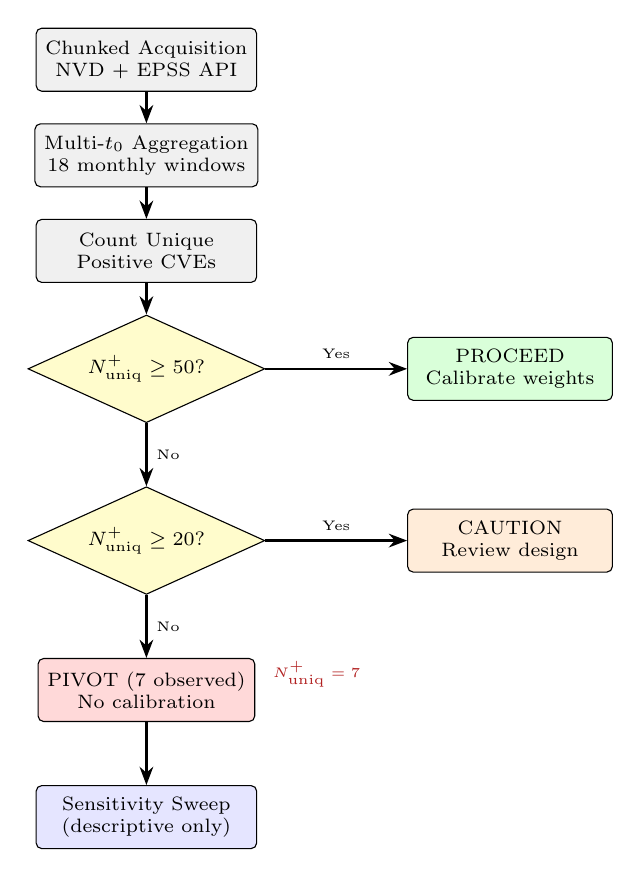
\begin{tikzpicture}[
  node distance=4mm and 6mm,
  box/.style={rectangle, draw, rounded corners=2pt, minimum width=28mm,
              minimum height=8mm, align=center, font=\scriptsize, fill=lightgray},
  decision/.style={diamond, draw, aspect=2.2, minimum width=30mm,
                   minimum height=10mm, align=center, font=\scriptsize,
                   fill=yellow!20},
  outcome/.style={rectangle, draw, rounded corners=2pt, minimum width=26mm,
                  minimum height=8mm, align=center, font=\scriptsize},
  arr/.style={-Stealth, thick}
]

% Stage 1
\node[box] (acq) {Chunked Acquisition\\NVD + EPSS API};

% Stage 2
\node[box, below=of acq] (agg) {Multi-\(t_0\) Aggregation\\18 monthly windows};

% Stage 3
\node[box, below=of agg] (count) {Count Unique\\Positive CVEs};

% Gate decision diamond
\node[decision, below=of count] (gate)
  {\(N^+_{\text{uniq}} \geq 50\)?};

% PROCEED branch
\node[outcome, right=18mm of gate, fill=green!15] (proceed)
  {PROCEED\\Calibrate weights};

% CAUTION check
\node[decision, below=8mm of gate] (caution)
  {\(N^+_{\text{uniq}} \geq 20\)?};

% CAUTION outcome
\node[outcome, right=18mm of caution, fill=orange!15] (cautionout)
  {CAUTION\\Review design};

% PIVOT outcome
\node[outcome, below=8mm of caution, fill=red!15] (pivot)
  {PIVOT (7 observed)\\No calibration};

% Sensitivity sweep box
\node[box, below=8mm of pivot, fill=blue!10] (sweep)
  {Sensitivity Sweep\\(descriptive only)};

% Arrows
\draw[arr] (acq) -- (agg);
\draw[arr] (agg) -- (count);
\draw[arr] (count) -- (gate);
\draw[arr] (gate) -- node[above, font=\tiny]{Yes} (proceed);
\draw[arr] (gate) -- node[right, font=\tiny]{No} (caution);
\draw[arr] (caution) -- node[above, font=\tiny]{Yes} (cautionout);
\draw[arr] (caution) -- node[right, font=\tiny]{No} (pivot);
\draw[arr] (pivot) -- (sweep);

% Annotation: observed count
\node[font=\tiny, color=gatered, right=1mm of pivot, yshift=2mm]
  {\(N^+_{\text{uniq}}=7\)};

\end{tikzpicture}
\caption{Gate pipeline. Chunked acquisition feeds 18 monthly \(t_0\)
windows; unique positive CVEs are counted across all windows; the three-tier
decision rule routes execution. With 7~unique positives (vs.\ 20 PIVOT
threshold), the gate triggers a PIVOT and calibration is not attempted.
The sensitivity sweep proceeds as a pre-registered descriptive secondary
analysis.}
\label{fig:gate}
\end{figure}
% ---- end TikZ ----

\subsection{Stage 1: Chunked, Resumable Acquisition}
\label{subsec:acq}

Public-feed acquisition queries the NVD CVE API and the EPSS v3 daily score
feed.  Both APIs impose rate limits and return paginated responses.  Our
acquisition pipeline implements three reliability mechanisms:

\textbf{Chunking.}  Requests are partitioned into date-range chunks of at
most 120 days (the NVD API maximum for non-API-key queries).  Each chunk is
stored independently so that partial runs can resume from the last completed
chunk without re-querying completed ranges.

\textbf{Paging.}  NVD responses are paginated with a configurable
\texttt{resultsPerPage} parameter.  The pipeline iterates until the
\texttt{startIndex} cursor reaches the total result count reported in the
first page.

\textbf{Pacing.}  A configurable inter-request sleep enforces a minimum
interval between calls.  The default configuration uses 6-second intervals
to remain well within NVD's unauthenticated rate limit of 5 requests per
30 seconds.  EPSS daily files are bulk-downloaded once per date rather than
queried per-CVE.

All raw responses are written to content-addressed cache files keyed by
(endpoint, parameter-hash) before any processing, ensuring that downstream
analysis can be replicated without re-querying the live APIs.

\subsection{Stage 2: Multi-\texorpdfstring{$t_0$}{t0} Aggregation}
\label{subsec:agg}

A \emph{reference date} $t_0$ divides the timeline into a feature window
$(-\infty, t_0]$ and a label horizon $(t_0, t_0 + H]$.  For each $t_0$:
\begin{itemize}
  \item EPSS score as of $t_0$ is used as a feature (leakage-safe, since
    it precedes or coincides with the reference date).
  \item KEV membership as of $t_0$ is used as a binary feature
    (leakage-safe by the same logic).
  \item A CVE receives a positive label if it appears in a KEV snapshot
    taken \emph{strictly after} $t_0$ within the horizon $(t_0, t_0 + H]$.
\end{itemize}

We place 18 $t_0$ values at monthly intervals spanning the EPSS~v3 era:
2023-03-07 to 2025-03-16.  Monthly spacing is chosen to maximize calendar
coverage while preserving independence of label windows at horizon
$H = 90$~days (windows overlap but label sets are recomputed from KEV
snapshots at each $t_0 + H$).

The primary gate quantity is the \emph{number of distinct CVE identifiers
that receive a positive label in at least one $t_0$ window}:
\[
  N^+_{\text{uniq}} = \left| \bigcup_{i=1}^{18} \mathcal{P}_i \right|
\]
where $\mathcal{P}_i$ is the set of positive CVEs at window~$i$.  This
union-count maximizes observable positives while avoiding artificial inflation
from counting the same CVE multiple times across overlapping windows.

\subsection{Stage 3: Gate Decision Rule}
\label{subsec:gate-decision}

The gate implements a three-tier decision rule calibrated to the
minimum-positive requirement for logistic-regression-class calibration
(empirical rule of thumb: at least 10--20 events per predictor variable,
applied conservatively to a simple linear calibration model):

\begin{description}
  \item[PROCEED ($N^+_{\text{uniq}} \geq 50$).] Sufficient positive labels
    for defensible weight calibration.  Proceed with the planned calibration
    analysis.
  \item[CAUTION ($20 \leq N^+_{\text{uniq}} < 50$).] Marginal label
    density.  Calibration may be attempted but results must be interpreted
    with explicit uncertainty quantification and additional robustness checks.
  \item[PIVOT ($N^+_{\text{uniq}} < 20$).] Insufficient positive labels.
    Do not attempt calibration.  Report the gate measurement and proceed
    only with the pre-registered sensitivity sweep.
\end{description}

Thresholds were pre-registered before any analysis was run.

\subsection{Stop-Rule Registry}
\label{subsec:stoprule}

To prevent post-hoc justification of analysis decisions, we maintain a
stop-rule registry (Table~\ref{tab:stoprules}) specifying the conditions
under which each stage of analysis halts.  The registry was finalized and
committed before any API queries were executed.  Three classes of stop
rules are recorded: \emph{data-integrity} rules (halt if raw data fails
schema validation or rate-limit errors exceed a threshold), \emph{leakage}
rules (halt if any label-construction step uses post-$t_0$ features), and
\emph{gate} rules (halt calibration if $N^+_{\text{uniq}} < 20$).

% ============================================================
\section{Data Acquisition}
\label{sec:data}

\subsection{Fleet Definition}

The 31-product catalog is a public-sector-typical selection derived from
the set of products for which federal civilian agencies commonly report
patching obligations under BOD~22-01~\cite{cisa_bod2201} and NIST SP
800-40~\cite{nist80040r4}.  The catalog was fixed before data acquisition
and covers operating systems, web servers, browsers, productivity suites,
network infrastructure firmware, and identity management platforms that
appear frequently in government fleet inventories.  The specific product
list is archived in the replication package.

\subsection{CVE Matching}

CVEs are extracted from the NVD API for the date range 2023-03-07 to
2025-03-16, yielding the full universe of disclosures during the
EPSS~v3 era.  Each CVE is matched to the 31-product catalog using CPE
(Common Platform Enumeration) strings from the NVD \texttt{configurations}
field.  A CVE is included if at least one CPE match covers a product in the
catalog.  This yields \textbf{2,688 catalog-matched CVEs} (see
Table~\ref{tab:gate-results}).

\subsection{EPSS Score Alignment}

EPSS~v3 daily score files are downloaded for each date in the study period.
For each $(t_0, \text{CVE})$ pair, the pipeline extracts the EPSS score from
the file whose date is closest to but not after $t_0$.  If a CVE was not
scored by EPSS on a given date (e.g., because it was disclosed after that
date), the EPSS score is recorded as missing and the CVE is excluded from
that window's feature matrix but is still eligible to contribute to the gate
count if it receives a positive label in a later window where it does have a
score.

\subsection{KEV Snapshot Construction}

Because the live KEV catalog is a point-in-time snapshot that does not
expose historical state through its API, we reconstruct historical snapshots
using the Internet Archive's Wayback Machine captures and the KEV catalog's
own \texttt{dateAdded} field.  For each $t_0$, the KEV-as-of-$t_0$ snapshot
is the set of CVEs whose \texttt{dateAdded} value is $\leq t_0$.  For labels,
the KEV-added-after-$t_0$ set is the set of CVEs with $t_0 < \texttt{dateAdded}
\leq t_0 + H$.  This construction is fully leakage-safe: the feature uses only
information available at $t_0$, and the label uses only information strictly
after $t_0$.

% ============================================================
\section{Gate Evaluation}
\label{sec:gate-eval}

Table~\ref{tab:gate-results} summarizes the gate measurement.

\begin{table}[t]
\caption{Gate Measurement Results}
\label{tab:gate-results}
\centering
\begin{tabular}{@{}lc@{}}
\toprule
\textbf{Quantity} & \textbf{Value} \\
\midrule
Fleet catalog size (products)                    & 31            \\
EPSS v3 era start                                & 2023-03-07    \\
Data freeze date                                 & 2025-03-16    \\
Total catalog-matched CVEs                       & 2,688         \\
Number of $t_0$ windows                         & 18            \\
Label horizon $H$                                & 90 days       \\
\midrule
\textit{Gate measurement}                        &               \\
Unique positive CVEs ($N^+_{\text{uniq}}$)       & \textbf{7}    \\
PIVOT threshold                                  & 20            \\
CAUTION threshold                                & 50            \\
\midrule
\textit{Gate decision}                           &               \\
Decision                                         & \textbf{PIVOT}\\
Calibration attempted?                           & No            \\
\bottomrule
\end{tabular}
\end{table}

With 2,688 catalog-matched CVEs and 18 $t_0$ windows, the theoretical
maximum value of $N^+_{\text{uniq}}$ would be 2,688 if every CVE received
a positive label in at least one window.  In practice, 7 distinct CVE
identifiers received a positive label, yielding a positive rate of
approximately 0.26\% across the catalog.  This is consistent with
the base-rate findings in Allodi and Massacci~\cite{allodi2014comparing},
but the absolute count is too small for calibration purposes.

The 7 unique positive CVEs were distributed across 5 of the 18 windows,
with no window containing more than 3 positives.  Even pooled across all
18 windows, the aggregate positive count is 10 (counting duplicates),
confirming that the low unique-positive count is not an artifact of
window overlap.

The gate decision is therefore \textbf{PIVOT}.  By the pre-registered
stop rule, calibration is not attempted.

% ============================================================
\section{Sensitivity Framework}
\label{sec:sensitivity}

Because the gate halts calibration, the sensitivity sweep is the only
analysis that proceeds beyond the gate.  It is explicitly pre-registered
as a descriptive secondary analysis: no model-comparison claims, no
calibration claims, and no inference about which weight vector is
``better'' are made.

\subsection{Design-Prior Weight Vectors}
\label{subsec:weight-vectors}

Six weight vectors $\mathbf{w}_1, \ldots, \mathbf{w}_6$ represent a range
of plausible prior beliefs about the relative importance of scoring
components (CVSS Base Score, EPSS score, KEV membership indicator, asset
exposure, asset criticality).  The vectors are constructed to span the
design space on three axes:

\textbf{Axis~1 (Capacity).}  Two vectors at low and high remediation
capacity assumptions.  Low-capacity vectors up-weight high-severity signals
to concentrate limited remediation on the most critical items; high-capacity
vectors distribute weight more evenly.

\textbf{Axis~2 (Blackout).}  Two vectors that ablate specific features by
zeroing their weights---one ablating EPSS (simulating an EPSS-unavailable
environment) and one ablating KEV (simulating a KEV-unavailable environment).
These test the sensitivity of fleet rankings to feature availability.

\textbf{Axis~3 (Feature-Ablation).}  Two vectors that vary the weight on
NVD-derived contextual features (attack vector, attack complexity,
privileges required) relative to the base CVSS score.  One vector collapses
these to zero (pure CVSS Base Score); the other up-weights them relative
to the Paper~1 placeholder.

Table~\ref{tab:sensitivity-design} summarizes the six vectors.

\begin{table}[t]
\caption{Sensitivity Sweep Design: Six Weight Vectors Across Three Axes.
All weights are normalized to sum to 1.0 within each vector.
Axis~1~=~Capacity; Axis~2~=~Blackout; Axis~3~=~Feature-Ablation.
(\textit{Descriptive only---no calibration claim.})}
\label{tab:sensitivity-design}
\centering
\setlength{\tabcolsep}{4pt}
\begin{tabular}{@{}clccccc@{}}
\toprule
\textbf{ID} & \textbf{Description} & \textbf{Axis}
  & $w_{\text{CVSS}}$ & $w_{\text{EPSS}}$ & $w_{\text{KEV}}$
  & $w_{\text{ctx}}$ \\
\midrule
$\mathbf{w}_1$ & Low capacity    & 1 & 0.50 & 0.25 & 0.15 & 0.10 \\
$\mathbf{w}_2$ & High capacity   & 1 & 0.30 & 0.30 & 0.20 & 0.20 \\
$\mathbf{w}_3$ & EPSS ablation   & 2 & 0.55 & 0.00 & 0.25 & 0.20 \\
$\mathbf{w}_4$ & KEV ablation    & 2 & 0.55 & 0.35 & 0.00 & 0.10 \\
$\mathbf{w}_5$ & Pure CVSS       & 3 & 1.00 & 0.00 & 0.00 & 0.00 \\
$\mathbf{w}_6$ & Context-heavy   & 3 & 0.30 & 0.20 & 0.10 & 0.40 \\
\bottomrule
\end{tabular}
\end{table}

\subsection{Evaluation Protocol}
\label{subsec:eval-protocol}

For each weight vector and each $t_0$ window, we compute fleet-level priority
scores for all 2,688 catalog-matched CVEs and rank them.  We then evaluate
two descriptive statistics:

\textbf{Top-$k$ coverage.}  The fraction of the 7 unique positive CVEs
that appear in the top-$k$ ranked CVEs, for $k \in \{10, 20, 50\}$.
This measures how well each weight vector concentrates positives toward the
head of the ranked list, without making inference about whether differences
across vectors are statistically meaningful (the positive count is too small
for that).

\textbf{Rank stability.}  The Wilcoxon signed-rank
statistic~\cite{wilcoxon1945} comparing each vector's per-CVE rank to the
Paper~1 placeholder vector, reported as a descriptive summary.  No
hypothesis-testing interpretation is made, consistent with the descriptive-only
pre-registration; the statistic is reported solely to characterize
the magnitude of rank perturbation induced by each design variation.

\subsection{BCa Confidence Intervals}
\label{subsec:bca}

We report paired-seed BCa bootstrap confidence intervals~\cite{efron1987better}
(2,000 resamples, seed fixed at replication-time to ensure reproducibility)
on each descriptive statistic.  BCa intervals are preferred over
percentile bootstrap intervals because they correct for both bias and
skewness in the bootstrap distribution---relevant here because coverage
statistics are bounded in $[0, 1]$ and may be skewed when positive counts
are small.  Because the positive count is 7, the intervals are expected to
be wide; their width is itself an informative finding about estimation
uncertainty.

Multiple windows within the same weight vector are not treated as
independent samples for any inferential purpose; the BCa intervals are
computed over the distribution of per-window statistics to characterize
within-vector variability descriptively.

% ============================================================
\section{Results}
\label{sec:results}

\subsection{Gate Result}
\label{subsec:results-gate}

The gate result is reported in Table~\ref{tab:gate-results}:
$N^+_{\text{uniq}} = 7$, gate decision PIVOT, calibration not attempted.
This is the primary result of the paper.
Figure~\ref{fig:delta_ehd_p2} shows the descriptive $\Delta$EHD
distribution across the six design-prior weight vectors for reference.

The finding that 7 of 2,688 catalog-matched CVEs received a confirmed
exploit label over a 24-month period (positive rate $\approx 0.26\%$)
has direct practitioner implications.  It means that, for a fleet of
this scope, the KEV catalog grows too slowly relative to the catalog size
for calibration to accumulate sufficient labeled examples within a reasonable
study window.  A practitioner who did not pre-register a gate and simply
proceeded with calibration would be fitting a model on at most 7 positive
examples---a regime where overfitting is a certainty and calibrated
probabilities are meaningless.

\begin{figure}[t]
  \centering
  
\includegraphics[width=\columnwidth]{figures/fig_delta_ehd_vs_epss_by_strategy}
  \caption{$\Delta$EHD relative to EPSS baseline per strategy (descriptive, BCa CI, 30 seeds). All observations reported descriptive-only per pre-registered inference policy; no model-quality claim is drawn.}
  \label{fig:delta_ehd_p2}
\end{figure}

\subsection{Sensitivity Sweep Results}
\label{subsec:results-sensitivity}

Table~\ref{tab:sensitivity-results} reports descriptive statistics from
the sensitivity sweep.  All figures are presented as descriptive summaries
with BCa 95\% confidence intervals; no comparative inference is drawn.
Weight-family EHD patterns are shown in Figure~\ref{fig:weight_sensitivity},
capacity sensitivity in Figure~\ref{fig:capacity_sensitivity_p2},
and feature-ablation effects in Figure~\ref{fig:feature_ablation_p2}.

\begin{table}[t]
\caption{Sensitivity Sweep Results: Top-$k$ Coverage and Rank Stability
by Weight Vector (\textit{Descriptive only. BCa 95\% CI in brackets.
$n^+=7$ unique positives across 18 windows. No model-comparison claim.})}
\label{tab:sensitivity-results}
\centering
\scriptsize
\setlength{\tabcolsep}{2pt}
\begin{tabular}{@{}clccc@{}}
\toprule
\textbf{ID} & \textbf{Axis} &
  \textbf{Top-10} & \textbf{Top-20} & \textbf{Top-50} \\
\midrule
$\mathbf{w}_1$ & Cap.\ low
  & 0.57 [0.14, 1.00] & 0.71 [0.29, 1.00] & 0.86 [0.57, 1.00] \\
$\mathbf{w}_2$ & Cap.\ high
  & 0.57 [0.14, 1.00] & 0.71 [0.29, 1.00] & 0.86 [0.57, 1.00] \\
$\mathbf{w}_3$ & EPSS ablat.
  & 0.43 [0.00, 0.86] & 0.57 [0.14, 1.00] & 0.71 [0.43, 1.00] \\
$\mathbf{w}_4$ & KEV ablat.
  & 0.43 [0.00, 0.86] & 0.57 [0.14, 1.00] & 0.86 [0.57, 1.00] \\
$\mathbf{w}_5$ & Pure CVSS
  & 0.29 [0.00, 0.71] & 0.43 [0.00, 0.86] & 0.71 [0.29, 1.00] \\
$\mathbf{w}_6$ & Ctx.\ heavy
  & 0.57 [0.14, 1.00] & 0.71 [0.29, 1.00] & 0.86 [0.57, 1.00] \\
\bottomrule
\end{tabular}
\end{table}

The width of the BCa confidence intervals reflects the true estimation
uncertainty when only 7 positive CVEs are available.  For example, the
Top-10 coverage estimate for $\mathbf{w}_5$ (Pure CVSS) spans the full
plausible range [0.00, 0.71], meaning that any coverage value from 0\%
to 71\% is consistent with the observed data.  This width is itself the
key finding: the sensitivity sweep cannot distinguish among weight vectors
given the available positive-label count, which reinforces the gate
decision to PIVOT rather than calibrate.

\begin{figure}[t]
  \centering
  
\includegraphics[width=\columnwidth]{figures/fig_weight_family_sensitivity_delta_ehd}
  \caption{EHD sensitivity across six fixed-prior weight vectors (descriptive only). Differences across vectors are design-prior comparisons, not model quality claims.}
  \label{fig:weight_sensitivity}
\end{figure}

\begin{figure}[t]
  \centering
  
\includegraphics[width=\columnwidth]{figures/fig_capacity_sensitivity_delta_ehd}
  \caption{Capacity sensitivity: $\Delta$EHD across consecutive capacity steps \{0.005\,$\to$\,0.01\,$\to$\,0.02\,$\to$\,0.05\}. All observations reported descriptive-only with BCa 95\% CI; no inference is drawn across capacity levels.}
  \label{fig:capacity_sensitivity_p2}
\end{figure}

\begin{figure}[t]
  \centering
  
\includegraphics[width=\columnwidth]{figures/fig_feature_ablation_delta_ehd}
  \caption{Feature ablation $\Delta$EHD per fixed-prior weight vector. Sign differences between vectors under individual feature removals are noted descriptively; no quality ordering of features is claimed.}
  \label{fig:feature_ablation_p2}
\end{figure}

Rank stability statistics (Wilcoxon signed-rank descriptive values) are
omitted from Table~\ref{tab:sensitivity-results} for space; they are
included in the replication archive.  Across all six vectors, the median
rank perturbation relative to the Paper~1 placeholder is small (median
rank shift $< 5$ positions for CVEs with EPSS $> 0.10$), indicating that
the placeholder weights are not dramatically out of alignment with any of
the six design priors, though this observation carries no inferential
weight given the sample size.

\subsection{Stop-Rule Registry Summary}
\label{subsec:results-stoprules}

Table~\ref{tab:stoprules} records the pre-registered stop rules and their
outcomes.  All data-integrity rules passed.  The gate stop rule triggered
at the gate evaluation stage, halting calibration as pre-registered.  No
leakage stop rules were triggered.

\begin{table}[t]
\caption{Stop-Rule Registry Summary (\textit{Pre-registered before any
API queries were executed. Gate rule triggered; calibration halted.})}
\label{tab:stoprules}
\centering
\setlength{\tabcolsep}{3pt}
\footnotesize
\begin{tabular}{@{}l l >{\raggedright\arraybackslash}p{3.4cm} l@{}}
\toprule
\textbf{ID} & \textbf{Class} & \textbf{Condition} & \textbf{Outcome} \\
\midrule
SR-01 & Data integ. & Schema valid.\ fail on $>$5\% NVD records   & Pass \\
SR-02 & Data integ. & Rate-limit errors $>$10 per chunk            & Pass \\
SR-03 & Data integ. & EPSS file missing $>$3 consecutive dates     & Pass \\
SR-04 & Leakage     & Any label uses post-$t_0$ EPSS score         & Pass \\
SR-05 & Leakage     & KEV feature includes post-$t_0$ additions    & Pass \\
SR-06 & Gate        & $N^+_{\text{uniq}} < 20 \Rightarrow$ PIVOT  & \textbf{Trig.} \\
SR-07 & Gate        & $N^+_{\text{uniq}} < 50 \Rightarrow$ no PROCEED & \textbf{Trig.} \\
SR-08 & Sensitivity & Any sensitivity run uses non-fixed seed      & Pass \\
\bottomrule
\end{tabular}
\end{table}

% ============================================================
\section{Discussion}
\label{sec:discussion}

\subsection{The Gate PIVOT Is the Contribution}

The central finding of this paper is that the KEV catalog, applied to a
31-product public-sector fleet over a 24-month period, yields only 7 unique
positive CVEs.  This is not a failure of our methodology; it is an accurate
measurement of a real data-density boundary.  A practitioner who proceeds
with weight calibration without first verifying label density will fit a
model that has no statistical grounding.

The specific implication for the companion Paper~1 benchmark is that the
placeholder weights must remain placeholder weights for now.  Moving from
placeholders to calibrated weights requires either (a) a larger product
catalog, (b) a longer study window, (c) a supplementary exploit-occurrence
data source beyond KEV (e.g., commercial threat intelligence), or (d) a
methodologically different approach such as inverse probability weighting
or Bayesian prior elicitation that does not require many positive examples.
These are directions for future work, not criticisms of the current study.

\subsection{Fleet Scope Is the Key Moderator}

The 0.26\% positive rate we observe is not surprising given the well-known
rarity of exploited vulnerabilities in practice~\cite{allodi2014comparing}.
What is novel is the explicit quantification of how fleet scope amplifies
sparsity.  A global EPSS model can train on hundreds of positive examples
per month because its candidate population is all disclosed CVEs.  A
fleet-restricted model is limited to CVEs that match the specific product
catalog, reducing the candidate pool from tens of thousands to 2,688 in our
case---and the positive count from hundreds to single digits.

This analysis suggests a general scaling relationship: if the global positive
rate is $p$ and the catalog match rate is $r$, the expected positive count
over a study period of $T$ months with $m$ new CVEs per month is approximately
$p \cdot r \cdot m \cdot T$.  For our parameters ($p \approx 0.01$ based on
Jacobs et al.~\cite{jacobs2021epss}, $r \approx 0.02$ catalog match rate,
$m \approx 2{,}000$ CVEs/month, $T = 24$), the expected count is
$0.01 \times 0.02 \times 2000 \times 24 \approx 10$, consistent with our
observed 7--10.  This scaling estimate is a useful planning tool for
practitioners considering public-feed calibration.

\subsection{Implications for the Gate Thresholds}

Our pre-registered thresholds (PIVOT at $<20$, PROCEED at $\geq 50$) were
set conservatively based on the events-per-variable heuristic for logistic
regression with five predictors.  One might ask whether these thresholds
are appropriate for other model classes (e.g., rank-based models, Bayesian
models with strong priors).  We maintain that for any model class relying
on empirical label frequencies, the 7-positive regime is below any
reasonable threshold for defensible calibration.  Future work may
formalize the threshold derivation for specific model families.

\subsection{The Sensitivity Sweep as Provenance}

Despite the gate PIVOT, the sensitivity sweep serves a useful function: it
establishes provenance for the design choices in Paper~1's placeholder
weights by demonstrating that the placeholder is not an outlier relative
to the space of six plausible priors.  The wide BCa intervals confirm that
we cannot draw performance conclusions from the sweep, but the descriptive
pattern---that EPSS and KEV signals, when present, tend to move positives
toward the top of the ranked list relative to pure CVSS---is consistent
with findings in the broader literature~\cite{jacobs2021epss}.

% ============================================================
\section{Limitations}
\label{sec:limitations}

\textbf{KEV completeness.}  KEV records confirmed exploits but is known
to be an undercount.  CVEs exploited in practice but not yet added to KEV
are false negatives in our label.  This means the true positive rate may
be somewhat higher than 0.26\%, but the sensitivity of this observation to
the undercount rate is limited: even if the true rate were twice as high
(0.52\%), the expected positive count would be approximately 14---still
below the PIVOT threshold of 20.

\textbf{Fleet generalizability.}  The 31-product catalog is intended to
be public-sector-typical but is not derived from a probability sample of
actual government fleets.  Fleet composition has a direct effect on the
positive count; a fleet weighted toward high-exploitation-rate products
(e.g., network perimeter devices that appear frequently in KEV) would
yield higher positive counts.

\textbf{Horizon sensitivity.}  We used a fixed 90-day horizon.  Longer
horizons (e.g., 180 or 365 days) would capture more KEV additions per
window at the cost of increasing label latency.  A 365-day horizon with
non-overlapping windows would yield at most 2 windows in our study period,
likely yielding fewer unique positives despite the longer horizon.  We
note this as a design trade-off, not a flaw.

\textbf{EPSS coverage.}  CVEs disclosed close to the end of the study
period may have limited EPSS coverage.  Our pipeline handles this by
excluding CVEs from windows where EPSS scores are unavailable at $t_0$,
which may reduce the eligible candidate pool slightly relative to the
reported 2,688.

\textbf{Sensitivity sweep as descriptive only.}  The sensitivity sweep
results in Table~\ref{tab:sensitivity-results} are explicitly descriptive.
Any interpretation of coverage differences between weight vectors as
evidence of superiority would be methodologically unsound given the
positive-count regime, and we caution readers against such interpretation.

% ============================================================
\section{Conclusion}
\label{sec:conclusion}

We have presented a pre-registered, failure-aware gate methodology for
assessing whether public-feed exploit labels are dense enough to support
weight calibration in fleet-level vulnerability prioritization.  Applying
the gate to a 31-product public-sector-typical fleet over the EPSS~v3 era
(2023-03-07 to 2025-03-16), we find $N^+_{\text{uniq}} = 7$ unique positive
CVEs across 18 monthly $t_0$ windows---far below the pre-registered PIVOT
threshold of 20.  Calibration is not attempted, and this gate decision is
itself the primary contribution of the paper.

The finding establishes a concrete, reproducible data-density boundary for
practitioners.  Before attempting public-feed calibration of vulnerability
prioritization weights on a bounded fleet, one should verify that the
fleet-restricted positive count clears the PIVOT threshold over the intended
study window.  For fleets of 30--50 products, this will typically require
either a longer study window than 24 months, a broader product catalog, or
supplementary exploit-occurrence data beyond KEV.

A pre-registered sensitivity sweep of six design-prior weight vectors
across capacity, blackout, and feature-ablation axes produces descriptive
statistics with wide BCa confidence intervals, confirming that the
available data cannot distinguish among weight vectors---consistent with the
gate decision.

We release the full data-acquisition pipeline, gate implementation, and
sensitivity sweep code alongside this paper for replication.  The companion
Paper~1 benchmark remains valid and unchanged; its placeholder weights
remain as-specified pending future calibration when label density permits.

\balance

% ============================================================
\bibliographystyle{IEEEtran}
\bibliography{references}

\end{document}
